\documentclass[%
 reprint,
%superscriptaddress,
%groupedaddress,
%unsortedaddress,
%runinaddress,
%frontmatterverbose, 
%preprint,
%showpacs,preprintnumbers,
%nofootinbib,
%nobibnotes,
%bibnotes,
 amsmath,amssymb,
 aps,
%pra,
%prb,
%rmp,
%prstab,
%prstper,
%floatfix,
]{revtex4-1}

\usepackage{graphicx}% Include figure files
\usepackage{dcolumn}% Align table columns on decimal point
\usepackage{bm}% bold math
%\usepackage{hyperref}% add hypertext capabilities
%\usepackage[mathlines]{lineno}% Enable numbering of text and display math
%\linenumbers\relax % Commence numbering lines

%\usepackage[showframe,%Uncomment any one of the following lines to test 
%%scale=0.7, marginratio={1:1, 2:3}, ignoreall,% default settings
%%text={7in,10in},centering,
%%margin=1.5in,
%%total={6.5in,8.75in}, top=1.2in, left=0.9in, includefoot,
%%height=10in,a5paper,hmargin={3cm,0.8in},
%]{geometry}

\usepackage{cmap} % Поиск в PDF
\usepackage[T2A]{fontenc} % Кодировка
\usepackage[utf8]{inputenc} % Кодировка исходного текста
\usepackage[english, russian]{babel} % Локализация и переносы
\frenchspacing % Более тонкая настройка пробелов 
\usepackage{multirow}
\usepackage[warn]{mathtext}
\usepackage{amssymb}
\usepackage{ dsfont }
\usepackage{ textcomp }
\usepackage{ mathrsfs }

% Переопределение англоязычного начертания каппа, фи и эпсилон, 
% а также знаков сравнения
\renewcommand{\epsilon}{\ensuremath{\varepsilon}}
\renewcommand{\phi}{\ensuremath{\varphi}} 
\renewcommand{\kappa}{\ensuremath{\varkappa}}
\renewcommand{\le}{\ensuremath{\leslant}}
\renewcommand{\leq}{\ensuremath{\leqslant}}
\renewcommand{\ge}{\ensuremath{\geslant}}
\renewcommand{\geq}{\ensuremath{\geqslant}}
\renewcommand{\emptyset}{\ensuremath{\varnothing}}

\usepackage{textcomp} 
\usepackage{indentfirst} % Красная строка
\usepackage{amsmath} % Текст в формулах
\usepackage{graphicx} % Графика
\DeclareGraphicsExtensions{.pdf,.png,.jpg}
\usepackage{pgfplots}
\pgfplotsset{compat=1.13}

%\usepackage{times}

\begin{document}

\title{Эффект Поккельса}
\thanks{4.7.2}

\author{Иван Едигарьев}
\affiliation{
 Московский Физико-Технический Институт\\
 Факультет Общей и Прикладной Физики, 526т\\
}
%\date{\today}

\begin{abstract}
Цель работы: исследовать интерференцию рассеянного света, прошедшего кристалл; наблюдать изменение характера поляризации света при наложении на кристалл электрического поля.

В работе используются: гелий-неоновый лазер, поляризатор, кристалл ниобата лития, матовая пластинка, экран, источник высоковольтного переменного и постоянного напряжения, фотодиод, осциллограф, линейка.\\

\end{abstract}

\pacs{Valid PACS appear here}% PACS, the Physics and Astronomy
                             % Classification Scheme.
%\keywords{Suggested keywords}%Use showkeys class option if keyword
                              %display desired
\maketitle

%\tableofcontent

\section{\label{sec:level1}Задание}

\begin{center}
I. Юстировка системы
\end{center}

\begin{figure}[h]
    \center{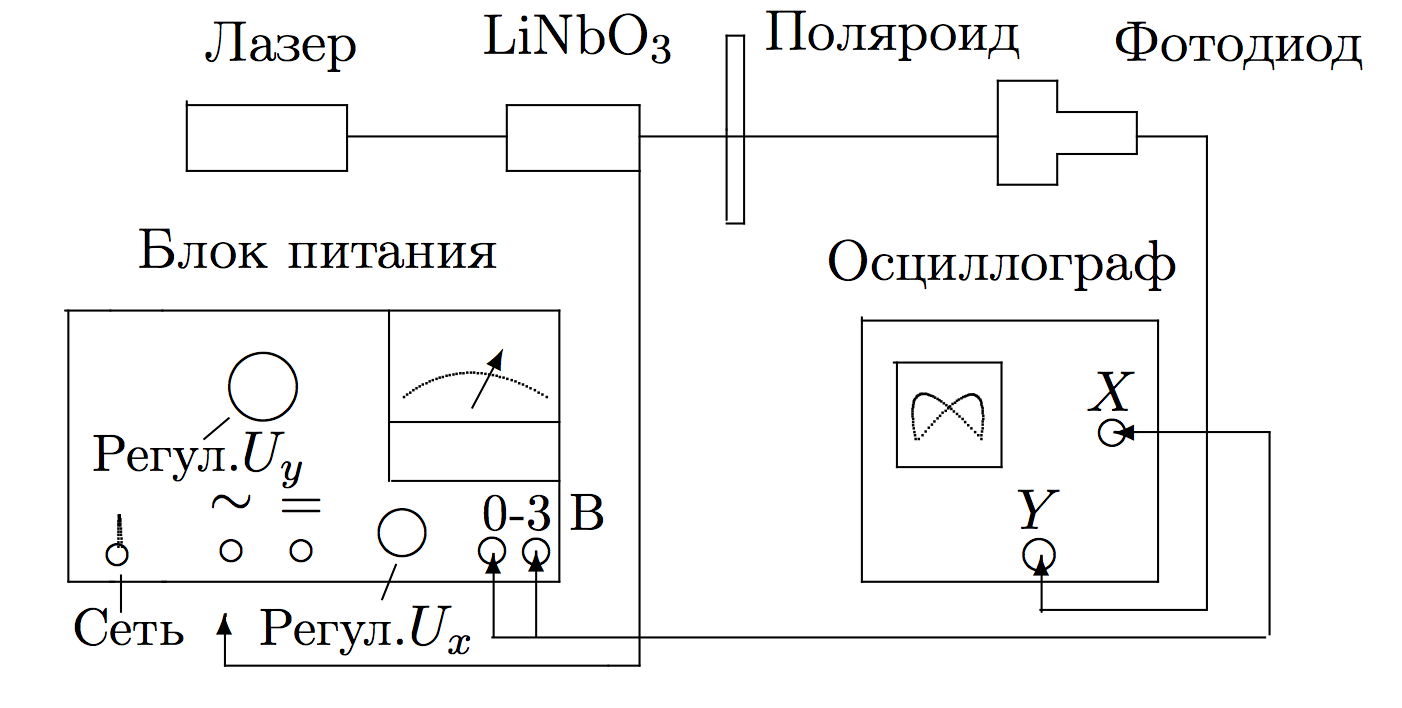
\includegraphics[scale=0.17]{pic1.png}}
    \caption{Схема для наблюдения интерференционной картины}
\end{figure}

\begin{enumerate}

    \item 
    Соберём оптическую схему согласно рис. 1. Включим лазер и установите анализатор (без кристалла в схеме) так, чтобы лазерное излучение через него не проходило (скрещенные поляризации).
    
    \item
    Поставим кристалл и установите перед ним вплотную к кювете матовую пластинку. Расстояние от кристалла до экрана определяет размер интерференционной картины и её контрастность.
    
    \item
    Получим на экране интерференционную картину. Отклоняя кристалл с помощью юстировочного винта (рис. 1) и поворачивая рейтер с кюветой вокруг вертикальной оси, добьёмся совмещения центра коноскопической картины с положением луча на экране в отсутствие матовой пластинки.
    
    \item
    Повернём анализатор на 90\textdegree~и убедимся, что коноскопическая картина изменилась на негативную. Вернём анализатор в прежнее положение (горизонтальное разрешённое направление).
    
\end{enumerate}

\begin{center}
I. Измерения
\end{center}

\begin{figure}[h]
    \center{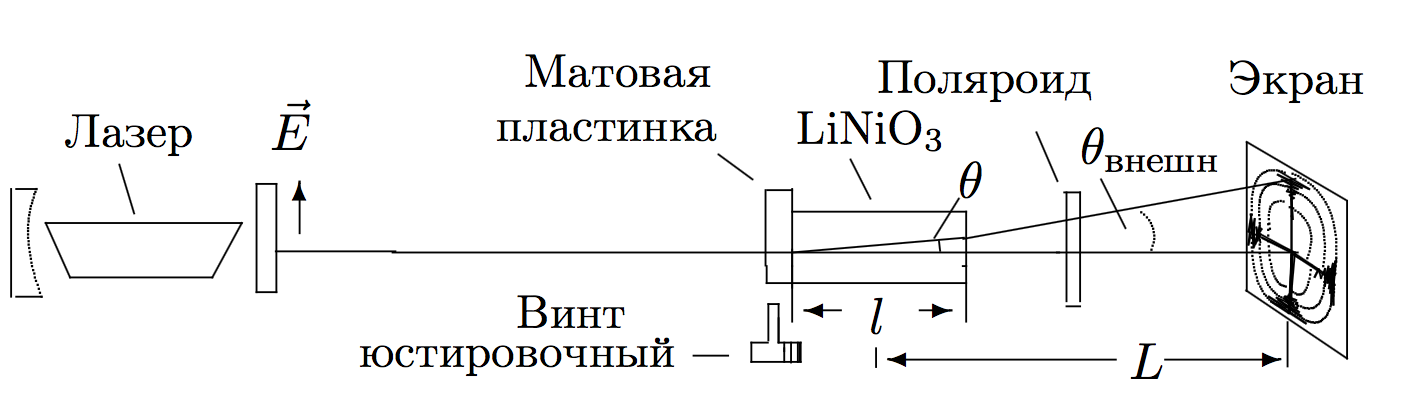
\includegraphics[scale=0.17]{pic2.png}}
    \caption{Схема для изучения двойного лучепреломления в электрическом поле}
\end{figure}

\begin{enumerate}
    \item
    Измерим радиусы тёмных колец $r(m)$ и расстояние $L$ от середины кристалла до экрана.
    $$ L = (75\pm 1)~cm$$
    
    Также запишем величины $n_0, l и \lambda$:
    \begin{gather*}
        n_0 = 2,29\\
        l = (2,7 \pm 0,3)~cm\\
        \lambda = 0,63~\mu m
    \end{gather*}
    
    Построим график $r^2 = f(m)$. По углу наклона прямой определим двулучепреломление $(n_0 - n_{\text{e}})$ ниобата лития.
    
    \begin{figure}[h]
    \center{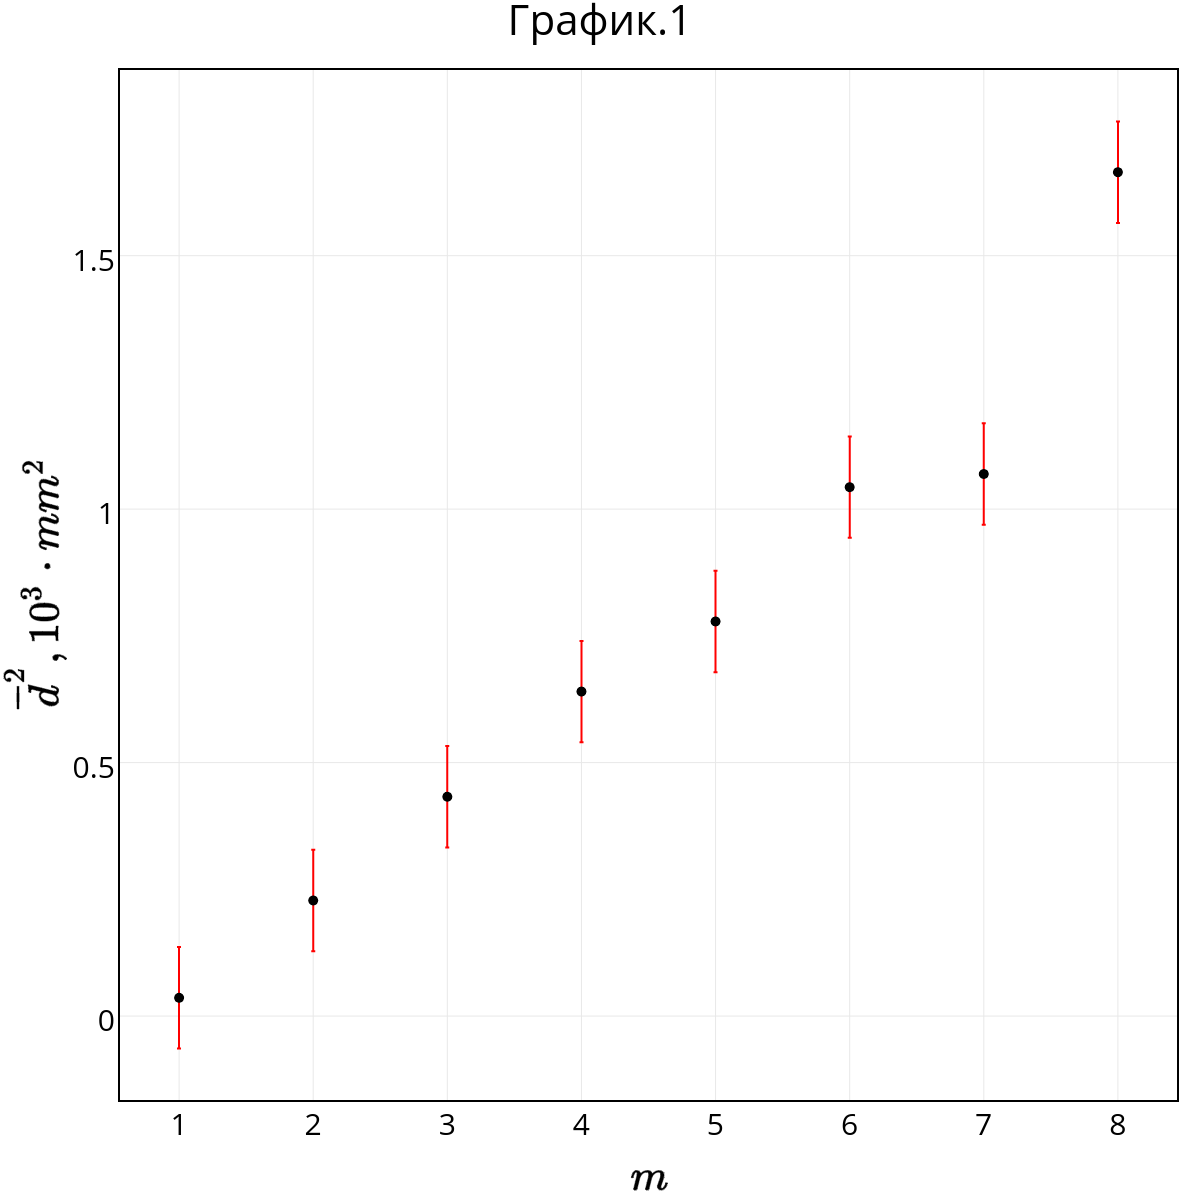
\includegraphics[scale=0.20]{my_plot1.png}}
    \end{figure}
    
    Построим двухпараметрический фит к модели:
    $$ y = \beta x + \alpha $$
    Будем считать распределние ошибок гауссовым и,  минимизируя функционал нормы $L2$, получим значения $\beta$ и $\alpha$, а также их оценочные дисперсии.
    \begin{gather*}
    \beta = (7.34\pm0.04^{\text{stat}})~{cm^2}\\
    \alpha = (2.3\pm0.2^{\text{stat}})~{cm^2}
    \end{gather*}
    
    Как можно видеть, $\alpha = 0.0$ не пренадлежит 95\% доверительному интервалу параметра $\alpha$
    
    $$(n_0 - n_{\text{e}}) = \frac{\lambda}{l} \frac{(n_0 L)^2}{\beta} = (0.937 \pm 0.005^{stat}\pm0.142^{syst})$$
    
    \item
    Ещё раз убедимся, что направление лазерного луча совпадает с направлением на центр интерференционной картины, и уберём матовую пластинку. 
    
    \item
    Подключим разъём блока питания на постоянное напряжение (=), установим регулятор напряжения на минимальное напряжение и включим блок питания в сеть.    
    
    \item
    С увеличением напряжения на кристалле яркость пятна на экране увеличивается и достигает максимума при $U = U_{\lambda/2}$. При $U = 2U_{\lambda/2} = U_\lambda$ яркость снова будет минимальной и т.д. Проделаем то же для параллельных поляризаций лазера и анализатора. Определим полуволновое напряжение ниобата лития.
    \begin{gather*}
    U_{\lambda/2}^{\perp} = (1035 \pm 30)~V\\
    U_{\lambda/2}^{\parallel} = (780 \pm 30)~V
    \end{gather*}
    
    \item
    Подадим на кристалл напряжение $U = \frac{1}{2}U_{\lambda/2} = U_{\lambda/4}$ (четвертьволновое напряжение). Поляризация на выходе кристалла должна быть круговой. Убедимся в этом, вращая анализатор и наблюдая за яркостью пятна на экране.
    
    \item
    Установим вместо экрана фотодиод (рис. 2) и подключим его к $Y$-входу осциллографа. Убрав напряжение до нуля, переключим разъём с постоянного (=) на переменное напряжение ($\sim$). С трёхвольтового выхода блока питания подадим сигнал на вход $X$ осциллографа. Отклонение луча осциллографа по оси $X$, таким образом, будет пропорционально напряжению $U$ на кристалле, а по оси $Y$-интенсивности прошедшего через анализатор сигнала $I_{\text{вых}}$.
    
    \item 
    Постепенно повышая напряжение на кристалле, пронаблюдаем на экране осциллографа фигуры Лиссажу, соответствующие зависимости $I_{\text{вых}}(U)$ для скрещенных поляризаций лазера и анализатора. Слегка поворачивая кристалл, сделаем фигуру Лиссажу симметричной. Определим по фигурам Лиссажу полуволновое напряжение $U_{\lambda/2}$ как $\Delta U$ , соответствующее переходу от максимума к минимуму сигнала на осциллограмме. Сравним значения полуволнового напряжения, полученные при постоянном и переменном напряжениях.
    \begin{gather*}
    U_{\lambda/2}^{\perp} = (855 \pm 30^{\text{syst} \pm 81})~V\\
    U_{\lambda/2}^{\parallel} = (735 \pm 30^{\text{syst}}\pm 35^{\text{stat}})~V
    \end{gather*}
    
    \item
    Зарисуем фигуры Лиссажу для напряжений $U_{\lambda/2}$, $U_{\lambda}$, $U_{3\lambda/2}$ при скрещенных поляризациях лазера и анализатора. Проследим, как меняется картина при переходе к параллельным поляризациям.

\end{enumerate}


\end{document}

